\documentclass[11pt]{article}
\usepackage[letterpaper,margin=0.82in]{geometry}
\usepackage{amsmath,amssymb,amsthm,mathtools,graphicx,microtype,xcolor}
\usepackage[colorlinks=true,linkcolor=blue!55!black,citecolor=blue!55!black,urlcolor=blue!55!black]{hyperref}

\newtheorem{theorem}{Theorem}
\newtheorem{proposition}[theorem]{Proposition}
\newtheorem{lemma}[theorem]{Lemma}
\newtheorem{remark}[theorem]{Remark}
\newcommand{\R}{\mathbb R}
\newcommand{\N}{\mathbb N}
\newcommand{\K}{\mathbb K}
\newcommand{\ip}[2]{\langle #1,#2\rangle}

\title{A kernel counterexample and the canonical repair\\
for the reverse Laplace polynomial inequality}
\author{Candidate counterexample and strengthened full result for arXiv:2502.07448}
\date{11 August 2026}

\begin{document}
\maketitle

\noindent\fbox{\parbox{0.95\linewidth}{\textbf{Status.}
Candidate full counterexample, likely valid, requiring human review.  The
printed conjecture is false because its left side annihilates constants while
its right side does not.  More substantially, the canonical repair obtained
by taking the right side modulo additive constants is true, with both
inequality directions.}}

\section{The printed conjecture and its repair}

Let
\[
 d\mu(x)=\tfrac12e^{-|x|}\,dx
\]
and let $(P_k)_{k\ge0}$ be its orthonormal polynomials, with $P_0=1$.
For $f\in L^2(\mu)$ put
\begin{equation}\label{eq:S}
 \mathcal S_\mu(f)=\sum_{k=1}^{\infty}
 \log^2(e+k)|\ip{f}{P_k}_{L^2(\mu)}|^2.
\end{equation}
Bizeul--Klartag prove an upper bound on \eqref{eq:S} and then conjecture
the reverse inequality shown below~\cite[p.~3]{BK}.

\begin{figure}[ht]
\centering
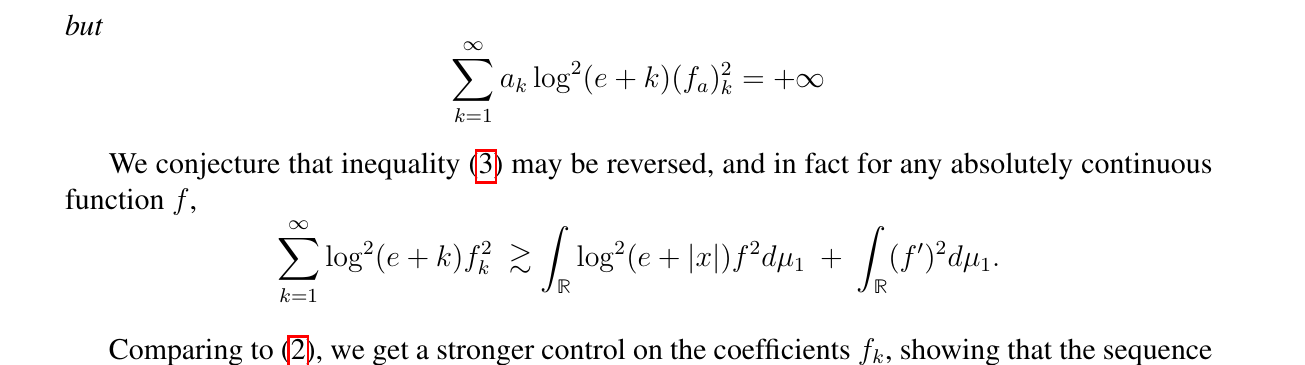
\includegraphics[width=0.97\linewidth]{figures/open_conjecture.png}
\caption{The conjecture in the source PDF.  Its quantifier is ``any
absolutely continuous function $f$''.}
\end{figure}

Thus the literal assertion is that, for some universal $c>0$ and every
absolutely continuous $f$,
\begin{equation}\label{eq:printed}
 \mathcal S_\mu(f)\ge c\left(
 \int_\R\log^2(e+|x|)|f(x)|^2\,d\mu(x)
 +\int_\R|f'(x)|^2\,d\mu(x)\right).
\end{equation}

\begin{proposition}[Counterexample to the printed conjecture]\label{prop:literal}
The inequality \eqref{eq:printed} is false.
\end{proposition}

\begin{proof}
Take $f\equiv1$.  Orthogonality gives $\ip{1}{P_k}=0$ for every $k\ge1$,
and $f'=0$, whereas
\[
 \int_\R\log^2(e+|x|)\,d\mu(x)>0.
\]
Hence the two sides of \eqref{eq:printed} are respectively zero and strictly
positive.
\end{proof}

The natural invariant replacement of the right side is
\begin{equation}\label{eq:Q}
 \mathcal Q_\mu(f)=\inf_{a\in\K}
 \int_\R\log^2(e+|x|)|f(x)-a|^2\,d\mu(x)
 +\int_\R|f'(x)|^2\,d\mu(x).
\end{equation}
Here and below $\K$ is $\R$ or $\mathbb C$.  This is not merely a way to
remove the counterexample: it gives the exact corrected theorem.

\begin{theorem}[Two-sided canonical repair]\label{thm:main}
There are universal constants $0<c\le C<\infty$ such that every absolutely
continuous $f$ satisfies
\begin{equation}\label{eq:equivalence}
 c\,\mathcal Q_\mu(f)\le \mathcal S_\mu(f)
 \le C\,\mathcal Q_\mu(f),
\end{equation}
with the usual extended-value interpretation.  Equivalently, the printed
conjecture becomes true after quotienting both sides by constants.
\end{theorem}

\subsection*{Proof intuition}
The source replaces the Laplace density, up to a dilation and bounded density
perturbation, by the hyperbolic-secant density.  There the orthonormal
Meixner--Pollaczek polynomials have an explicit generating function.  Its
$x$-derivative turns differentiation into a one-sided Hilbert matrix; a
dyadic near/far split costs exactly one logarithm.  Multiplication by $x$
becomes the Jacobi matrix with off-diagonal entries $n+1$.  A short limiting
interpolation argument then transfers the graph bound for this Jacobi matrix
to a logarithmic graph bound.  These two estimates prove the new direction
$\mathcal Q\lesssim\mathcal S$; the other direction is the source theorem
applied after subtracting an arbitrary constant.

\section{The hyperbolic-secant model}

Let
\begin{equation}\label{eq:nu}
 d\nu(x)=\frac{dx}{2\cosh(\pi x/2)}.
\end{equation}
The source records the generating function
\begin{equation}\label{eq:generating}
 G(x,z)=\frac{e^{x\arctan z}}{\sqrt{1+z^2}}
 =\sum_{n=0}^{\infty}p_n(x)z^n,\qquad |z|<1,
\end{equation}
where $(p_n)_{n\ge0}$ is an orthonormal basis of $L^2(\nu)$~\cite[Sec.~1.1]{BK}.
Differentiating \eqref{eq:generating} in $z$ and in $x$ gives
\begin{align}
 xp_n&=(n+1)p_{n+1}+np_{n-1}, \label{eq:recurrence}\\
 p_n'&=\sum_{\substack{1\le r\le n\\r\ \mathrm{odd}}}
 \frac{(-1)^{(r-1)/2}}{r}\,p_{n-r}. \label{eq:derivative}
\end{align}
We use these identities to control both terms in \eqref{eq:Q}.

\begin{lemma}[Derivative estimate]\label{lem:derivative}
For every finite scalar sequence $(c_n)$,
\begin{equation}\label{eq:derivative-bound}
 \left\|\left(\sum_{n\ge0}c_np_n\right)'\right\|_{L^2(\nu)}^2
 \le C\sum_{n\ge1}\log^2(e+n)|c_n|^2.
\end{equation}
\end{lemma}

\begin{proof}
By \eqref{eq:derivative} and orthonormality, the coefficient of $p_m$ in the
derivative is
\[
 (Tc)_m=\sum_{\substack{n>m\\n-m\ \mathrm{odd}}}
 \frac{\varepsilon_{n-m}}{n-m}c_n,
 \qquad |\varepsilon_{n-m}|=1.
\]
Let $c^{(j)}$ be the restriction of $c$ to
$I_j=[2^j,2^{j+1})\cap\N$, for $j\ge0$.  Split $Tc^{(j)}$ into the near
part $m\ge2^{j-1}$ and the far part $m<2^{j-1}$, with the evident convention
for $j=0$.

For the near part, Young's convolution inequality and the harmonic-sum bound
give
\[
 \|(Tc^{(j)})_{\rm near}\|_2
 \le \left(\sum_{1\le r\le2^{j+1}}\frac1r\right)\|c^{(j)}\|_2
 \le C(j+1)\|c^{(j)}\|_2.
\]
Its output is supported in $[2^{j-1},2^{j+1})$, so these output supports have
uniformly bounded overlap as $j$ varies.  Hence the squared norm of the sum
of all near parts is at most
$C\sum_j(j+1)^2\|c^{(j)}\|_2^2$.

For the far part, its Hilbert--Schmidt norm is uniformly bounded because
\[
 \sum_{n\in I_j}\sum_{m<2^{j-1}}\frac1{(n-m)^2}\le C.
\]
Therefore
\begin{align*}
 \left\|\sum_j(Tc^{(j)})_{\rm far}\right\|_2
 &\le C\sum_j\|c^{(j)}\|_2\\
 &\le C\left(\sum_j(j+1)^2\|c^{(j)}\|_2^2\right)^{1/2},
\end{align*}
where the last step uses $\sum_j(j+1)^{-2}<\infty$.  Since
$j+1\asymp\log(e+n)$ on $I_j$, combining the two parts proves
\eqref{eq:derivative-bound}.
\end{proof}

We next isolate the logarithmic interpolation fact used for the spatial
weight.

\begin{lemma}[Logarithmic graph interpolation]\label{lem:log-interpolation}
Let $A,B\ge I$ be positive self-adjoint operators on a Hilbert space.  If
$D(B)\subseteq D(A)$ and
\begin{equation}\label{eq:graph}
 \|Au\|\le M\|Bu\|\qquad(u\in D(B)),
\end{equation}
then
\begin{equation}\label{eq:log-graph}
 \|(I+\log A)u\|\le C_M\|(I+\log B)u\|.
\end{equation}
\end{lemma}

\begin{proof}
For $T\ge I$, use the quadratic $K$-functional
\[
 K_T(t,u)=\inf_{u=u_0+u_1}
 \big(\|u_0\|^2+t^2\|Tu_1\|^2\big)^{1/2}.
\]
The spectral theorem and scalar minimization give
\[
 K_T(t,u)^2=\int_{[1,\infty)}
 \frac{t^2\lambda^2}{1+t^2\lambda^2}\,d\|E_T(\lambda)u\|^2.
\]
For every $\lambda\ge1$, splitting the $t$-integral at $1/\lambda$ shows
\begin{equation}\label{eq:K-log}
 1+\int_0^1\log(1/t)
 \frac{t^2\lambda^2}{1+t^2\lambda^2}\,\frac{dt}{t}
 \asymp (1+\log\lambda)^2.
\end{equation}
Thus the integral of $K_T(t,u)^2$ in \eqref{eq:K-log}, plus $\|u\|^2$,
is equivalent to $\|(I+\log T)u\|^2$.

Condition \eqref{eq:graph} gives $K_A(t,u)\le K_B(Mt,u)$.  Substitute
$s=Mt$ in the integral.  On $0<s<1$, the extra constant $\log M$ is
controlled by the same integral plus $\|u\|^2$; on $1\le s\le M$, use
$K_B(s,u)\le\|u\|$.  Applying \eqref{eq:K-log} for $A$ and $B$ proves
\eqref{eq:log-graph}.
\end{proof}

\begin{lemma}[Spatial logarithm]\label{lem:spatial}
For every finite scalar sequence $(c_n)$,
\begin{equation}\label{eq:spatial-bound}
 \int_\R\log^2(e+|x|)\left|\sum_{n\ge0}c_np_n(x)\right|^2d\nu(x)
 \le C\sum_{n\ge0}\log^2(e+n)|c_n|^2.
\end{equation}
\end{lemma}

\begin{proof}
On $\ell_2(\N_0)$ let $J$ be the Jacobi operator corresponding to
\eqref{eq:recurrence}, and let $Be_n=(n+1)e_n$.  Thus the polynomial
transform takes $J$ to multiplication by $x$.  Directly from the two shifts,
\[
 \|Jc\|_2^2\le4\|Bc\|_2^2.
\]
Set $A=(I+J^2)^{1/2}$.  Then $A,B\ge I$ and
\[
 \|Ac\|_2^2=\|c\|_2^2+\|Jc\|_2^2\le5\|Bc\|_2^2.
\]
Lemma~\ref{lem:log-interpolation} applies.  Finally, on the spectral side,
the scalar functions
\[
 \log(e+|x|),\qquad 1+\log\sqrt{1+x^2}
\]
are comparable, while on coefficients
$1+\log(n+1)\asymp\log(e+n)$.  This is exactly
\eqref{eq:spatial-bound}.
\end{proof}

\section{Return to the Laplace measure}

We use an elementary comparison principle already exploited in the source.
If probability measures $\alpha$ and $\beta$ satisfy
$c\beta\le\alpha\le C\beta$, then their best polynomial approximation
errors are comparable.  If $(a_k^\alpha)$ and $(a_k^\beta)$ are the
coefficients of the same $f$ in their respective orthonormal polynomial
bases, then
\[
 \sum_{k\ge n}|a_k^\alpha|^2\asymp
 \sum_{k\ge n}|a_k^\beta|^2.
\]
For any increasing sequence $w_k$ with $w_0=0$, summation by parts gives
\[
 \sum_{k\ge1}w_k|a_k|^2
 =\sum_{n\ge1}(w_n-w_{n-1})\sum_{k\ge n}|a_k|^2.
\]
Consequently the coefficient sums with
$w_k=\log^2(e+k)$ are comparable.

Under the dilation $y=\pi x/2$, the measure \eqref{eq:nu} becomes
\[
 d\rho(y)=\frac{dy}{\pi\cosh y}.
\]
Its density and $\tfrac12e^{-|y|}$ are bounded above and below by universal
multiples of each other.  The dilation and this density comparison also
preserve, up to universal constants, the derivative norm and
\[
 \inf_a\int_\R\log^2(e+|y|)|f(y)-a|^2\,d\rho(y).
\]

\begin{proof}[Proof of Theorem~\ref{thm:main}]
In the $\nu$ model, subtract the constant coefficient $c_0$ from
$f=\sum c_np_n$.  Lemmas~\ref{lem:derivative} and~\ref{lem:spatial} give
\[
 \inf_a\int\log^2(e+|x|)|f-a|^2d\nu+\int|f'|^2d\nu
 \le C\sum_{n\ge1}\log^2(e+n)|c_n|^2.
\]
The dilation and comparison principle transfer this inequality to $\mu$,
proving the left inequality in \eqref{eq:equivalence}.  The estimates extend
from polynomials by completion; multiplication by the spatial weight and
weak differentiation are closed operators.

For the other direction, apply Theorem~1 of the source to $f-a$.  Its
positive-degree coefficients and derivative do not depend on $a$, so taking
the infimum over $a$ proves
$\mathcal S_\mu(f)\le C\mathcal Q_\mu(f)$.
\end{proof}

\section{Verification, sharpness, and novelty boundary}

The source's unpublished reverse-proof draft, still present as commented
source code in arXiv:2502.07448v1, contains the false step
\[
 \sum_{k\ge1}|f_k|^2\ge\int|f|^2d\nu,
\]
which is precisely the missing constant coefficient exposed by
Proposition~\ref{prop:literal}.  The June 17, 2025 authors' version and the
December 2025 journal publication still print the literal conjecture on PDF
page 3.

As a non-proof stress test, the Jacobi and derivative matrices were truncated
at five doubling dimensions from 16 through 256, with 512 padding modes for spectral
quadrature.  The largest generalized eigenvalue of the repaired right side
against the logarithmic coefficient form stayed between $1.9954$ and
$1.9956$.  At dimension 512 the spatial and derivative pieces separately
had largest ratios about $1.6494$ and $0.7704$.  The reusable script is
included as \path{code/finite_section_probe.py}.

There is also an exact high-frequency check.  For $f_t(x)=e^{itx}$ under
$\nu$, \eqref{eq:generating} and the transform
$\int e^{ux}d\nu(x)=1/\cos u$ give
\[
 \ip{f_t}{p_n}=\operatorname{sech}(t)\,[i\tanh(t)]^n.
\]
Thus the squared coefficients form a geometric law of typical degree
$e^{2|t|}$, and their logarithmic energy is comparable to $t^2$, matching
$\|f_t'\|_2^2=t^2$.  This confirms the sharp logarithmic scale.

The four run indexes had no prior entry for this paper or conjecture.  Bounded
searches through 11 August 2026 used the arXiv id, the exact conjecture phrase,
the title with ``reverse inequality'', the authors with
``Meixner--Pollaczek'', and later citations.  They found no correction or
answer.  Both the constant observation and the repaired theorem could be
folklore or independently known; no priority claim is made.

\paragraph{Human-review recommendation.}
First confirm that the published quantifier really includes constants.  For
the strengthened theorem, independently check the $K$-functional identity
\eqref{eq:K-log}, the scale change in Lemma~\ref{lem:log-interpolation}, and
the coefficient-tail comparison under bounded density perturbations.  The
dyadic derivative estimate is otherwise elementary.

\begin{thebibliography}{9}

\bibitem{BK}
P.~Bizeul and B.~Klartag,
\emph{Polynomial approximation in $L^2$ with the double-sided exponential
weight via complex analysis},
Journal of Approximation Theory \textbf{312} (2025), 106218;
arXiv:2502.07448v1.

\end{thebibliography}

\end{document}
